\section{Introduction}
\label{industry_needs}
As we mentioned in chapter \ref{chapter_general_intro}, the aim of this thesis has been twofold: deriving a methodology for inferring the motivational state of individuals while interacting with potentially rewarding object (a videogame in this case) and presenting how this could be used in an applied setting.

In this view, this chapter will focus on sketching the design of a system relying on our methodology for automated engagement prediction. First we will introduce a set of ethical considerations that should be taken into account when designing such system. Subsequently, we will provide an overview on why an industry player (or groups thereof) might need a process for quantifying and predicting engagement and which characteristics this process should have. Finally we will proceed at illustrating a system designed for serving this need, placing particular emphasis on how its components connect with the work presented so far.

\section{Some Ethical Consideration}
\label{ehtical_considerations}
Automated system leveraging behavioural data are now-days used extensively in both low and high stakes scenarios \cite{mehrabi2021survey}, with the potential to have a direct and concrete impact on individuals. For this reason, when designing automated data-driven applications, issues related to fairness should be taken into account. 

By fairness we entail the set of principles and considerations that in recent years are adopted in order to avoid that decisions based on a machine-learned model do not inadvertently bring harm to specific groups of people \cite{mehrabi2021survey}. A complete overview of the issue of fairness in machine learning would be beyond the scope of not just this section but the entire thesis, as it is a vast landscape \cite{mehrabi2021survey} hard to navigate due to its many levels of complexity \cite{corbett2018measure}.  We will therefore focus on three major aspects related to the work presented in this chapter. 

The first aspect concerns biases present in the data on which a machine learning algorithm is fitted. These might be induced by an over or under representation of certain strata of the population that an automated system will ultimately need to serve \cite{mehrabi2021survey}. Given how a large part of machine learning algorithms are fitted to the data (e.g., maximum likelyhood) the risk is that the prediction produced by the algorithm will revert to the mean or in the worst case, will result to be biased with respect to the true characteristics of the population \cite{corbett2018measure, mehrabi2021survey}. Despite the harm that these biases might cause in the context of engagement prediction is not as pronounced as in other areas (e.g., credit, criminal or medical risk assessment), they can still have unexpected repercussion on an individual if they assume that people engage in similar ways regardless of situational, personal and cultural differences. For example an individual might receive notifications in inappropriate contexts (e.g.,  during an emotionally challenging period) or be unfairly penalized within the game world (e.g., due to irregular playing patterns caused by personal or situational reasons) because they deviate from what is the expected behaviour in the data on which the algorithm was fitted.

To this connects the second aspect of fairness that we want to highlight, namely the risk of inadvertently cause harm to individuals which are either temporarily or structurally subject to some form of vulnerability. This might happen as a consequence of automated decision making based on what we call "unconstrained model predictions", what we mean by this is when the predictions from a model are used verbatim without knowing the context in which they will be applied. For example, if we imagine a system aimed at individuating high spending users within a game relying on gacha or loot-box mechanics, relying on unconstrained predictions might in this case inadvertently target individuals with a predisposition to or an history of problematic gambling behaviour \cite{petrovskaya2022prevalence}. The most problematic aspect related of this issue is that often the information required for "constraining" an "unconstrained prediction" are not available to the system, either because they are not easy to derive (e.g., they are not directly observable) or should not be accessible (e.g., they are Personal Identifiable Information - PII \cite{EUdataregulations2018}).

Related to the first two points is the third and final aspect of fairness that we would like to address which is connected with the right to object specified by the General Data Protection and Regulation act (GDPR) \cite{EUdataregulations2018} which allows an individual to object to the processing of their data in any form and at any moment. Despite this aspect is partially attenuated by rights granted by the GDPR (although this interests exclusively the European Union), it only covers the processing of data rather than the effect connected with automated decision making. An individual might object to the inclusion of their data during the decision making process but still be subject to the effect of this last one, for example if the system entails a policy of blanket intervention based on the average user behaviour for all those individuals for which no data are available.

As we mentioned at the beginning of the paragraph, an exhaustive treatment of these issues and the relative mitigating actions that could be taken is beyond the scope of the current work. Nevertheless we want to stress that addressing them in an effective manner is of pivotal importance when automated systems based on machine-learning (or other form of statistical decision making) becomes part of the operations of an industry player.

\section{Autometed Engagement Quantification and Prediction in a Videogame Setting}
\label{industry_needs}
As we mentioned before, in an industry setting the development of research projects often aims at the the resolution of specific problems or at the improvement of processes central to its success (being it measure in terms of revenues or perceived quality of goods and services). So where does engagement quantification and prediction sits within the needs of the videogame industry? Very often (if not always) the success of a videogame title is strictly connected with either its ability to retain users or with the experience that users had with the product. The first is pivotal in scenarios where games are treated as a service sold to an audience (similarly to the function of streaming services) while the second is more relevant in situations where games are considered digital goods. 

In this context, engagement can be viewed as a measure of how a particular game was, is or will be able to retain users: if an individual is engaged with a particular service it is likely that will keep take advantage of it similarly if an individual had a particular good experience and gladly engaged with a particular digital good it is is more likely that will either suggest it to other users, acquire similar products or buy product from the same seller.  

In this view being able to estimate the propensity that a user has towards a particular game translates (in a more or less direct way) to the capacity of assessing if a game is likely to be a success of public and revenue. For this reason it is often the case that videogame publishers and studios try to leverage the information they have available through telemetry system for taking the stock of how a particular game is performing. This is the classical example of analytical reports summarizing various type of game related Key Performance Indicators \cite{el2016game} 

\section{System Design Diagram}
\label{pipeline}
In this section we will briefly outline 

\section{Data Generation}
This is the first component of the system and describes the entities generating the data which will then be used by the system. It is composed by the major elements: the users and the game contexts. The relationship between these two entities has already been partially described in chapter \ref{chapter_lit_review} and \ref{chapter_theory_modelling} in particular and we can say that is 

\subsection{Users}
\lorem
\subsection{Game Contexts}
\lorem

\section{Model Owner}
This components represents the entity responsible for the acquisition ad storage of data generated by the interaction of the users with the game context. This entity is also in charge in managing the algorithm used for deriving a model from the data. It is relevant to highlight that the model owner usually corresponds one-to-one with the entity managing the game contexts but the two don't necessarily  have to coincide. In the context of federated learning  \cite{yang2019federated} for instance, a model owner might distribute copies of a learning algorithm across separate entities and only act as a pooling mechanism  once they have been fitted to the data \cite{kairouz2021advances}. In this case, these entities don't necessarily need to be known by the model owner and in fact must often be kept hidden as the aim of federated learning is to generate global and robust model fitted on multi-source data while being compliant with strict privacy constrains \cite{yang2019federated, kairouz2021advances}. That said, in this section we will focus on a situation in which the model owner is one with the game contexts owner.

\subsection{Data Storage}
\lorem
\subsection{Model Generation}
\lorem
\paragraph*{Data Generators} \lorem
\paragraph*{Model Configurations} \lorem
\paragraph*{Model Tuning} \lorem
\paragraph*{Model Training} \lorem
\paragraph*{Model Validation} \lorem
\paragraph*{Model Serving} \lorem

\section{Model Consumer}
\lorem
\subsection{Representation Sharing}
\lorem
\subsection{Profile Generation}
\lorem
\subsection{Live Predictions}
\lorem
\subsection{Automated Reporting}
\lorem

\begin{figure}[ht]
\centering
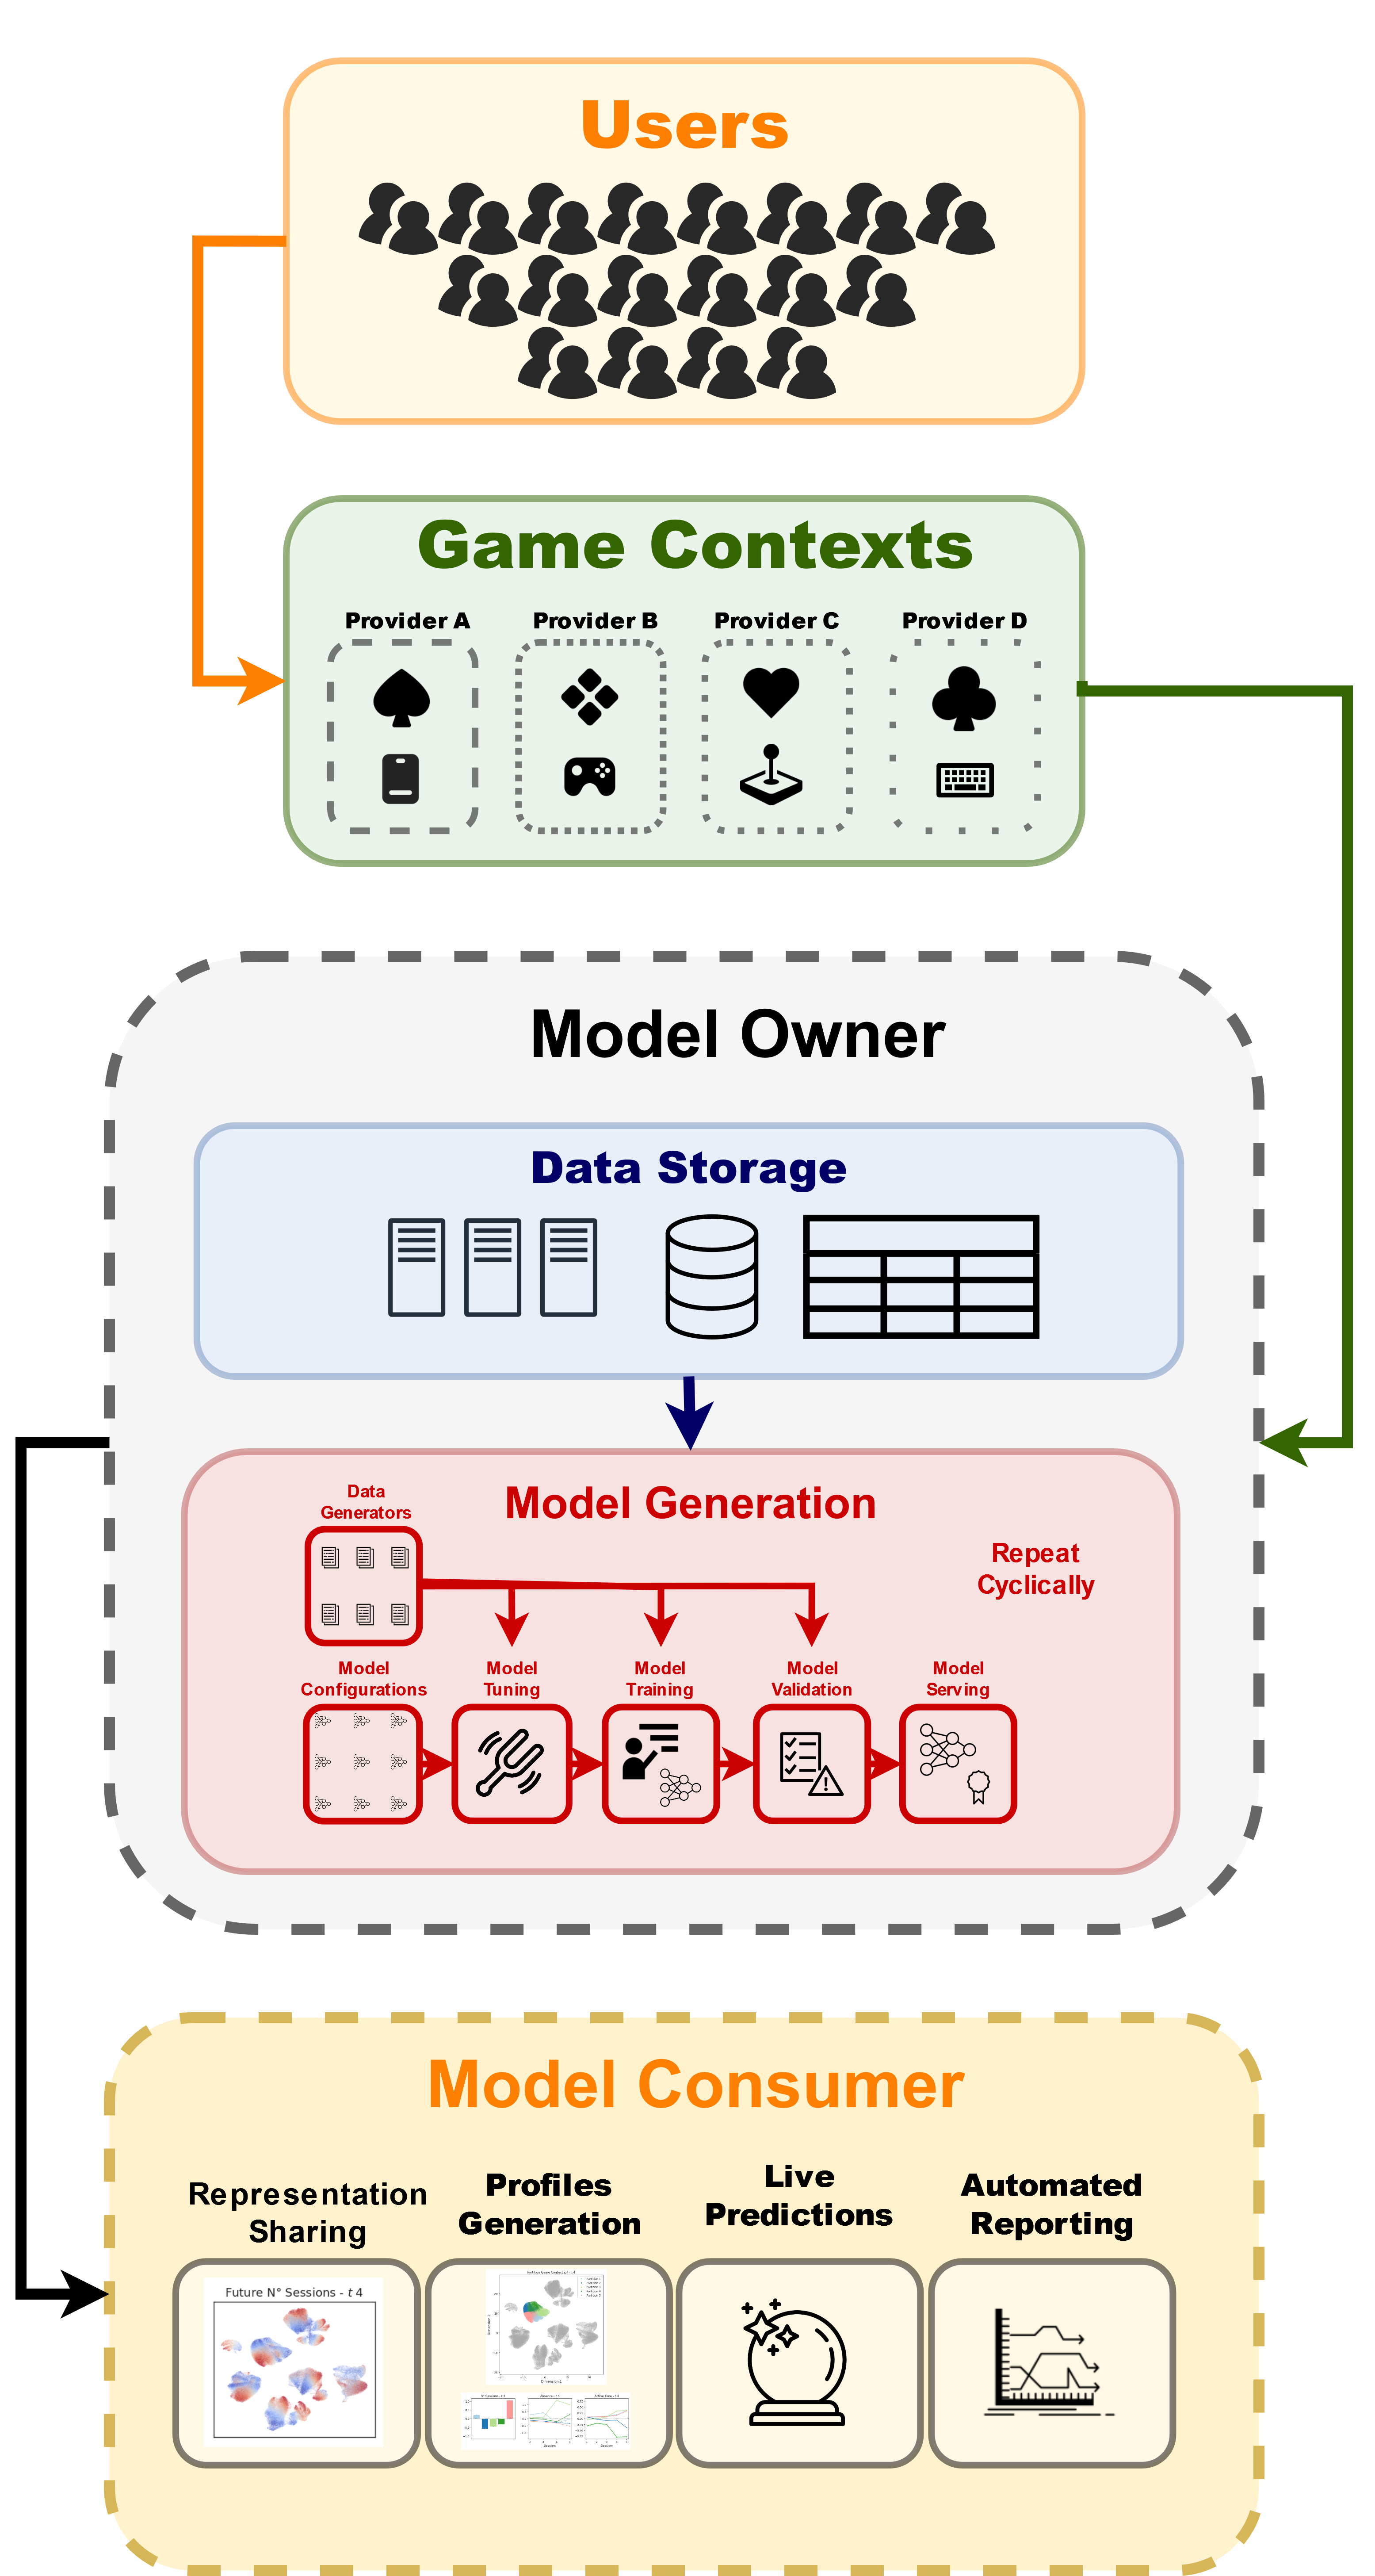
\includegraphics[width=0.7\textwidth]{images/chapter_5/pipeline_diagram.png}
\caption[\textbf{Model Deployment Pipeline}]{The figure represents a simplified system diagram for a potential application of the improved RNN architecture. Solid lines represent low-level components in the system while dashed lines indicate high-level entities. Directional arrows represent the flow of operations inside the system.}
\label{pipeline}
\end{figure}